%!TEX root = pixel-wise-street-segmentation.tex

\section{Evaluation}\label{sec:evaluation}

In the following section we will discuss the evaluation and results of our approaches. First, we will evaluate our different approaches. Second, we will compare our best one to the work of Mohan [~\cite{Tarel2009}]  (which is ranked on place 1 at KITTI road segmentation [~\cite{Tarel2009}]).
As already stated, the KITTI Road Estimation dataset the basis for our evaluation.\\
To be able to try out and evaluate our different approaches we used only the training data of the KITTI data set, as the ground truth for the test data is not publicly available. We splitted the training data beforehand 20 to 80 (test/training) in order to be able to measure our performance. 
Our best approaches with the parameter which worked best we submitted on the KITTI official evaluation website [link to website]


Our personal goal was to achieve an adequate classification performance while staying within a time frame of \textbf{20 ms} as maximal classification time per image. Resulting in a possible real time application usability of our approach, which would be the use case for street classification in autonomous cars anyway.\\

We used a computer with these specifications for the evaluation the GPU was used for training and testing):
\begin{itemize}
\item Intel(R) Core(TM) i7-4790K CPU @ 4.00GHz
\item System memory 16 GiB
\item GeForce GTX 980 4GiB Ram
\end{itemize}

Table \ref{tab:ownapproach} shows the result of our evaluation and regression approach using the models and parameters as described in section [MODEL]. The used score is the F1-measure \ref{eq:fMeasure} which is also used for the KITTI evaluation.
The table also shows the values of true positive (TP), true negative, false positive (FP), false negative (FN) and accuracy (ACC) \ref{eq:accuracy} with the red coloured number being the best one in this column. This gives a better insights if pixels tend to be more wrongly correct or false classified . It shows clearly that the regressions has an overall better F1-measure and accuracy score than the classification approach. Surprisingly a smaller stride does not automatically lead to a better performance. In the classification approach a stride with the size of 37 gets the best result while in the regression based approach a stride of 51 (patch size) achieves the best performance. Unfortunately the ram of the graphic card limited our possibility to use larger patch sizes. This could have been a good way to train and evaluate on full image size and still keep our time constraint\\

\begin{equation} \label{eq:fMeasure}
F1-measure = \frac{2*TP}{2TP +FP +FN}
\end{equation}
\begin{equation} \label{eq:accuracy}
accuracy = \frac{TP + TN}{TP + FP + TN + FN}
\end{equation}

\begin{table}[h!]
  \begin{center}
    \label{tab:ownapproach}
    \begin{tabular}{c|cccccc}
    \toprule
      \textbf{Netztyp} & {\bf F1} & \textbf{TN} & \textbf{FP} & \textbf{FN} & \textbf{TP} & \textbf{ACC} \\
       \midrule
      \textbf{Reg. - Stride 10} & 0.880 & 0.977 & 0.022 & 0.197 & 0.802 & 0.947\\
      \textbf{Reg. - Stride 37} & 0.890 & 0.973 & 0.026 & 0.176 & 0.823 &  \textcolor{red}{0.948}\\ 
      \textbf{Reg. - Stride 51} & \textcolor{red}{0.895} & 0.969 & 0.030 & 0.165 & \textcolor{red}{0.834} & 0.946\\
      \midrule
      \textbf{Kla. - Stride 10} & 0.854 & 0.981 & 0.018 & 0.241 & 0.758 & 0.942\\
      \textbf{Kla. - Stride 37} & 0.862 & 0.959 & 0.040 & 0.212 & 0.787 & 0.929\\
      \textbf{Kla. - Stride 51} & 0.701 & \textcolor{red}{0.982} & 0.017 & 0.451 & 0.548 & 0.906\\
      \bottomrule
    \end{tabular}
    \caption{Results on our approaches with different strides (S) on our own test set (58 images, ~ 6,7 mil. pixels)}
  \end{center}
\end{table}

To evaluate if we could meet our predefined goal (doing the classification in under 20 ms) we did a run time evaluation which is shown in table \ref{tab:runtime}. As expected the runtime increase with a lower stride size. The classification approach shows an overall faster run time as the regression. Finally, we managed to achieve a run time under 20 ms by using a stride of 51 in both approaches.



 \begin{table}[h!]
  \begin{center}
  \label{tab:runtime}
    \begin{tabular}{c|ccc}
    \toprule
      \textbf{network type/stride} & \textbf{10} & \textbf{37} & \textbf{51} \\
     \midrule
      \textbf{regression} & 1.99 & 0.29 & 0.18 \\
      \textbf{classification} & 1.83 & 0.2 & 0.11\\
      \bottomrule
    \end{tabular}
        \caption{Runtime per image (621x188 pixel) in seconds.}
  \end{center}
\end{table}


As the regression approach had the best performance and also met our time constraint we used it to evaluate the KITTI test set and submitted the results after a transformation into birds eye view (KITTI specifications). Table \ref{tab:kitti} shows the results which are split into the different road types (UM, UMM, UU, URBAN).
Unfortunately our approach performs much worse on the official test set then on our own test set. Here the F1-measure score ranges between 0.564 and 0.797 while Mohan achieves on all road categories a F1-measure score over 0.9. The reason for this huge difference to might be: \\
1.overfitting on our own test set data\\
2. we specialised our models and also our patch size on images with half the original size the KITTI evaluation was done on full size images\\
3. as seen in the following images {fig:badimages}

      \begin{table}[h!]
  \begin{center}
  \label{tab:kitti}
\begin{tabular}{c|cccccc}
 {\bf Benchmark} & {\bf F1} & {\bf AP} & {\bf PRE} & {\bf REC} & {\bf FPR} & {\bf FNR}\\ \hline
UM\_ROAD & 67.91 \% & 61.63 \% & 86.90 \% & 55.74 \% & 3.83 \% & 44.26 \%\\
UMM\_ROAD & 79.67 \% & 78.41 \% & 93.29 \% & 69.51 \% & 5.50 \% & 30.49 \%\\
UU\_ROAD & 56.48 \% & 51.89 \% & 84.67 \% & 42.37 \% & 2.50 \% & 57.63 \%\\
URBAN\_ROAD & 71.10 \% & 65.14 \% & 89.83 \% & 58.84 \% & 3.67 \% & 41.16 \%\\
\end{tabular}
  \end{center}
\end{table}




\begin{figure}[p]
    \centering
    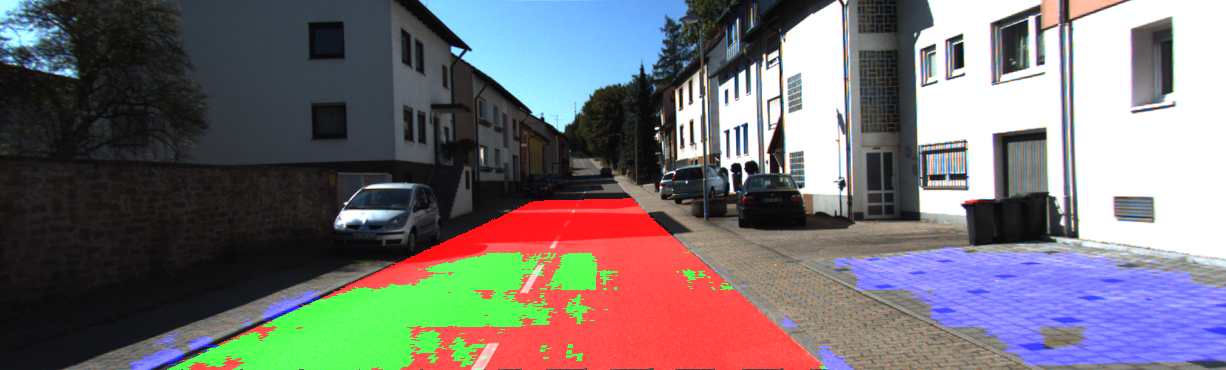
\includegraphics[scale=0.18]{figures/kitty_eval/Persp_um_road_000077.png}
    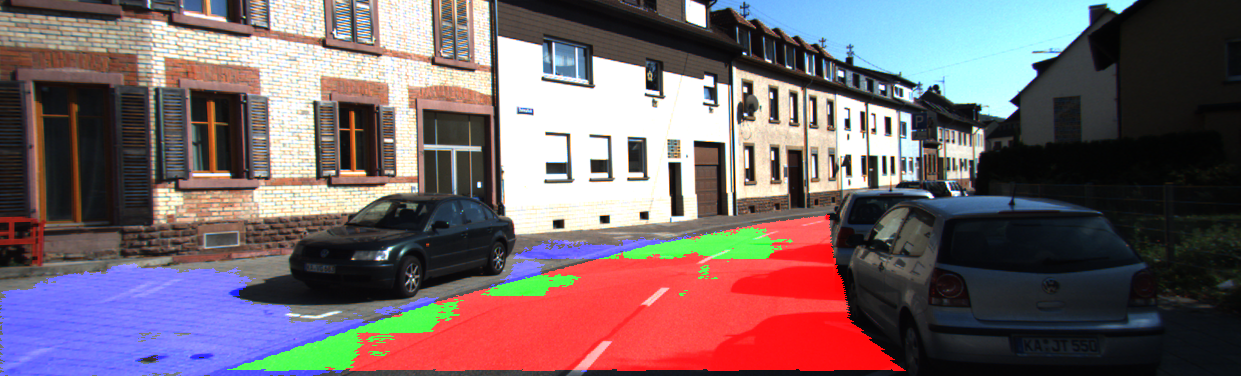
\includegraphics[scale=0.18]{figures/kitty_eval/Persp_um_road_000095.png}
    \caption{Here, red denotes false negatives, blue areas correspond to false positives and green represents true positives. }
    \label{fig:badimages}
\end{figure}




%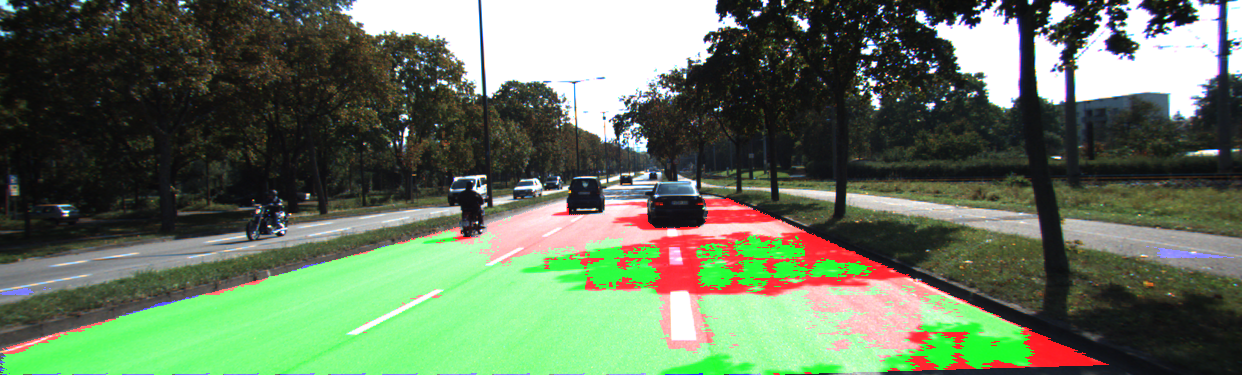
\includegraphics[scale=0.2]{figures/kitty_eval/Persp_umm_road_000025.png}
%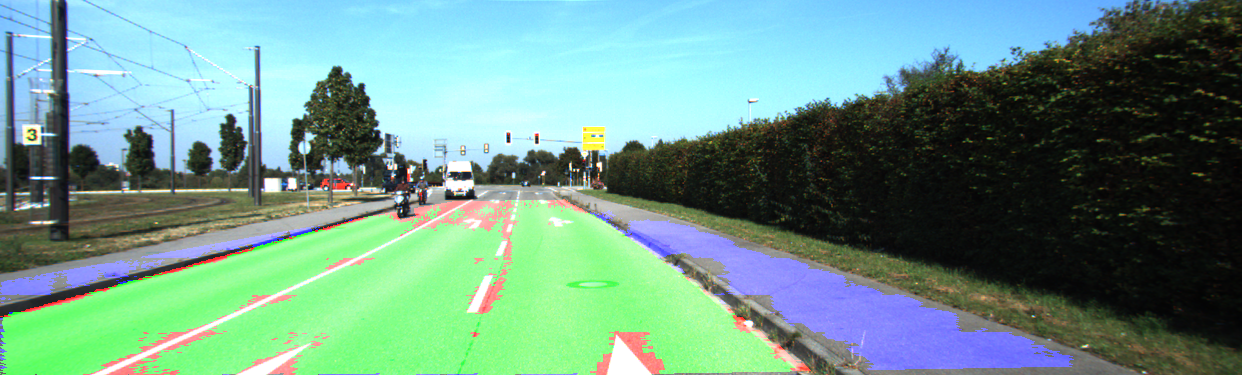
\includegraphics[scale=0.2]{figures/kitty_eval/Persp_umm_road_000040.png}
%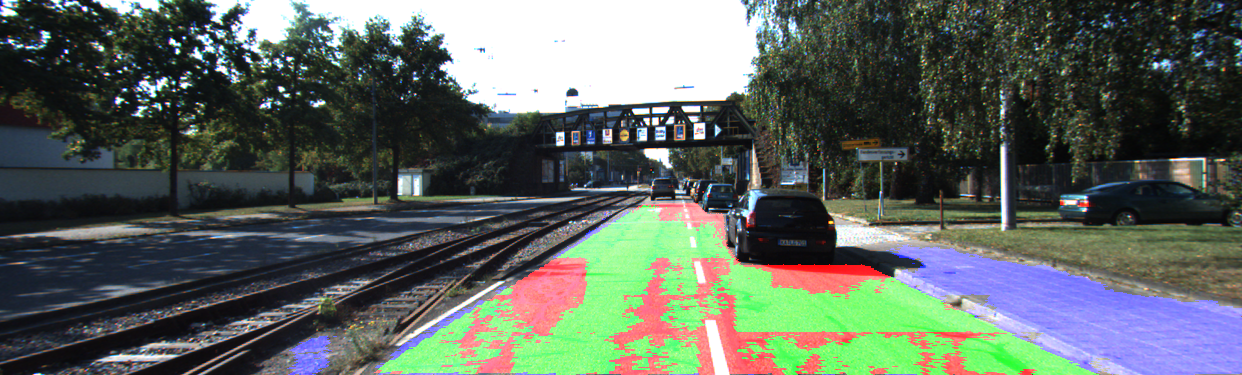
\includegraphics[scale=0.2]{figures/kitty_eval/Persp_umm_road_000066.png}
%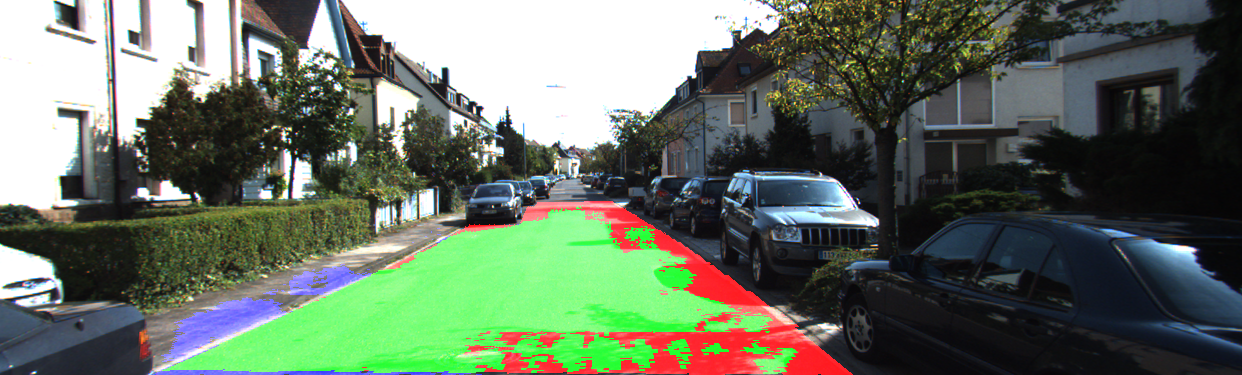
\includegraphics[scale=0.2]{figures/kitty_eval/Persp_uu_road_000020.png}

\begin{figure}[p]
    \centering
    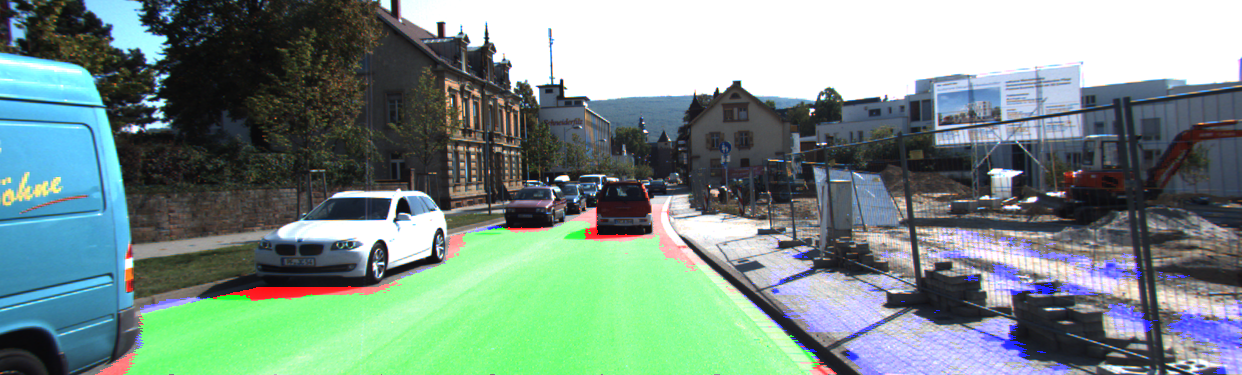
\includegraphics[scale=0.2]{figures/kitty_eval/Persp_uu_road_000027.png}
	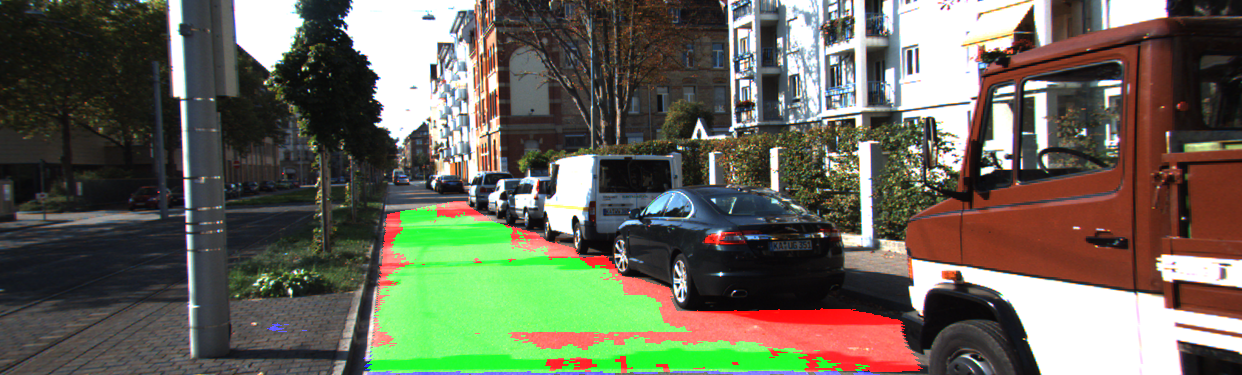
\includegraphics[scale=0.2]{figures/kitty_eval/Persp_uu_road_000082.png}
    \caption{Here, red denotes false negatives, blue areas correspond to false positives and green represents true positives. }
    \label{fig:badimages}
\end{figure}






%
